\documentclass[edit,11pt,ChapStyle3,twoside,doubleinterligne]{ManuscriptThese}

%%%%%%%%%%%%%%%%%%%
\usepackage{ParStartThese}
\usepackage{FontsThese}
\usepackage{UtilsThese}

\usepackage{eurofont}
%%%%%%%%%%%%%%%%%%%
%\usepackage[frenchb]{babel}
\usepackage[pdftex]{graphicx}

\usepackage{float}
\usepackage{url}
\usepackage{makeidx}

\usepackage[T1]{fontenc}
\usepackage[latin1]{inputenc}

\usepackage{amsmath, amsthm, amssymb}

%where to find the figures
\graphicspath{ {figs/} {StateoftheArt/figs/} }

%%%%%%%%%%%%%%%%%%%
% custom commands

%Insert a definition =>  \defintion{title}{content}
\newcommand{\definition}[2]{
   \begin{quotation}	\parbox{0.9\textwidth}
		{\textbf{Definition -  #1: }#2}
  \end{quotation} 
} 

%%%%%%%%%%%%%%%%%%%
%%%%%%%%%%%%%%%%%%%
%%%%%%%%%%%%%%%%%%%

\makeindex
\author{\@ThesisAuthorFirstName \@ThesisAuthorLastName}
\title{\@ThesisTitle}

\begin{document}

%-------------------------------------------------------------------
%                         Page de titre:
%-------------------------------------------------------------------
% La page de titre se compose automatiquement avec la commande
% \MakeThesisTitlePage
% Certains champs ont des valeurs par d\'efaut (Th\`ese pr\'esent\'ee \`a...),
% valeur qui d\'epende du style utilis\'e (rennes1, ou brest)
%
% l'exemple suivant fait le tour des commandes modifiables

%\newcommand{\MakeThesisSynthesisPage}%
%{%
%  \newpage
%  \@cover@hook
%  \thispagestyle{empty}
%  \begin{changemargin}{-1.5cm}{-1cm}
%    \thesissynthesispgebody
%  \end{changemargin}
%  \newpage  
%  \if@twoside
%  \thispagestyle{empty}
%  \hbox{}
%  \par\vfill
%  \newpage
%  \addtocounter{page}{-2}%
%  \else
%  \addtocounter{page}{-2}%
%  \fi
%  \fontencoding{OT1}\normalfont\selectfont
%  }%
%\newcommand\thesissynthesispgebody{%
% %---------------------------------------------------
%  \if@doubleinterligne\renewcommand\baselinestretch{1.0}\fi
%  %\vspace*{2cm} 
%  %
%  %POUR DECALER VERS LE BAS LA PAGE DE TITRE%
%  \begin{center}
%    \vfill
%    \Large\@ThesisAuthorFirstName\space\@ThesisAuthorLastName
%    \vfill
%    \textsc{\textbf{\@ThesisTitle}}
%    \vfill
%    \normalsize\normalfont Directeur de thse :
%    \vfill
%    \@ThesisSupervisorFirstName\space\@ThesisSupervisorLastName, \@ThesisSupervisorTitle
%    \vfill
%    \textbf{-- Rsum --}
%    \input{chapitre0/resume}
%  \end{center}
% %---------------------------------------------------
%  }

\NumeroOrdre{}

\ThesisMention{Informatique}

\ThesisTitle{A Multiagent System based Framework for Optimization} 

%\ThesisAbbrv{Le titre court de ma thse}

\ThesisDate{28th Febuary 2013}

\ThesisAuthorFirstName{Tom}

\ThesisAuthorLastName{Jorquera}

\ThesisSupervisorFirstName{Marie-Pierre}

\ThesisSupervisorLastName{Gleizes}

\ThesisSupervisorTitle{DR}

\EquipeAccueil = {Systèmes Multi-Agents Coopératifs}

\LaboratoireAcceuil = {Institut de Recherche en Informatique de
Toulouse}

\EcoleDoctorale= {Informatique et Télécommunication}

\CompositionDuJury{
  \begin{center}
  \UseEntryFont{ThesisCompositionJury}

  \begin{tabular}{lll}
    \multicolumn{3}{c}{\textsc{Jury}\vspace{0.5em}}\\
    Michle \textsc{Dupont} & \emph{Professeure, Universit de Toulouse III} & (prsidente du jury)\\
    \\
    Anne \textsc{Durand} & \emph{Professeure, Universit de Caen} & (rapporteure)\\
    \multicolumn{3}{c}{\textsc{Invit}\vspace{0.5em}}\\
    Marc \textsc{Duval} & \emph{MCF, Universit de Toulouse III} & (co-encadrant)\\
  \end{tabular}
  \end{center}
}
\def\blanc{\hspace*{.5cm}}

% Creation de la page de titre:
\MakeThesisTitlePage


%\input{Prelude/PagesResumes}

%\begin{ThesisDedication}
%\input{Prelude/Dedicace}
%\end{ThesisDedication}

%\newpage
%\thispagestyle{plain}
%\input{Prelude/Remerciements}

\Sommaire

\Introduction{Introduction} \label{introduction}
%\Introduction{Introduction} \label{introduction}

\section*{Complex Continuous Optimization and Multi-Agent Systems}

Continuous optimization is a very large field including various methods tailored for diverse specific requirements. While this approach was successful in providing a toolbox of specialized methods, the evolution of industrial needs draws attention to some of its limitations. Indeed, current optimization methods fail to handle the more complex optimization problems. These problem are characterized by heavy calculus, the many interdependencies between their components and the diverse expertise domains they involve. Classical optimization tools struggle with these problems because of these factors, and specific methods have been proposed to handle this complexity, giving birth to the field of Multidisciplinary Design Optimization (MDO). However,  MDO methods involve possibly important transformations to the original problem in order to divide the problem into simpler ones, which make this approach somewhat cumbersome and potentially inefficient for highly connected problems.

At the same time, new paradigms are being proposed to handle systemic complexity. One of the most successful is the field of Multi-Agent Systems (MAS). This approach proposes to handle problem complexity using systems of interconnected agents. Instead of reducing the problem in order to solve it using a centralized process, MAS techniques preserve the original problem and use decentralized mechanisms in order to spread the solving effort among the agents. MAS has proved successful in the field of combinatorial optimization, on problems such as graph coloring, sensors network or scheduling.

During the last ten years, the scientific community has relentlessly pursued the effort to bridge the gap between these two apparently irreconcilable approaches: mathematical optimization and MAS. The goal of this thesis is to contribute to this effort by addressing this mostly unexplored potential application field of MAS: complex continuous optimization.

\section*{Contributions of the Thesis}

The main contribution of this thesis concerns the applicability of MAS for continuous optimization We study continuous optimization problem and show how all of them share a common structure. Using this observation, we propose a representation of continuous optimization problems entities graphs, which we call Natural Domain Modeling for Optimization (NDMO). Based on this representation we identify several agent roles for the graph entities. For each agent role we propose a nominal behavior in order to produce a MAS capable of distributing the optimization process. In accordance with the AMAS theory, we identify a set of Non-Cooperative Situations (NCSs) susceptible to disturb the normal optimization process, and propose a set of cooperation mechanisms to handles them. We demonstrate the modularity of our system by introducing additional concerns with the handling of uncertainties propagations.

This thesis also provides two smaller contributions concerning the deisgn of MAS.  First of all, using the Make Agent Yourself framework  we propose a component-based architecture for AMAS adapted to the handling of multiple agent roles and NCS-related mechanisms. This architecture is based on the idea of stackable skills components following the hierarchy of agent roles, providing the correct methods at the required level.

We also provide a more theoretical contribution by abstracting the NCS and solving mechanisms into more general Collective Problem Solving Patterns (CPSP). These CPSP are based on a more high-level agent role representation, and are abstracted from any direct application domain. They represent specific agent topologies which can be encountered in agent organizations leading to a disruption of the correct system function, as well as of solving mechanisms proposed to handle such configurations. We propose a schematic \enquote{blueprint} representation which synthesize the content of the different patterns.

\section*{Manuscript Organisation}
This thesis is divided into 4 parts:
\begin{enumerate}[P{a}rt I.] %the {a} avoids this letter to be used as the counter (the I is used instead)
\item This part introduces the context of the study by presenting an overview of the continuous optimization field, MAS for optimization and the Adaptive Multi-Agent Systems theory.
\item This part presents the contribution of this thesis: a MAS for solving continuous optimization problems. We propose a modeling of a continuous optimization problem as an agent graph, and describe some cooperative behaviors for the different agent roles.
\item [[TODO: depends on CPSP chapter]].
\item In this part we present the experiments we did in order to evaluate and validate our approach.
\end{enumerate}

%%%%%%%%%%%%%%%%%%%

%\Partie{Ma première partie}


\chapter{State of the Art}

\section{Optimization}

\subsection{Basic Concepts}

Before starting to present the different categories of optimization and some related existing methods, we would like to take some time defining what exactly optimization is. In the more general way, optimizing is \emph{trying to find the best element among an element set} (when finding this best element is not trivial, we can rightfully talk of \emph{solving an optimization problem). }This somewhat simple definition implies in fact quite a lot.

First of all it implies we have a defined set of element to choose from. As we will see, the topology of the set is in fact of the utmost importance for solving the problem. This set of element is often named the \emph{search space}, \emph{solution space} or \emph{domain}. In {}``simple'' optimization problems, the search space can be simply defined by a set of elements (for example \{a,b,c\} or \ensuremath{\mathbb{R}}) associated with a set of \emph{constraints}. For large problems, the search space can be defined by calculus-heavy equations, empirical models, complex algorithms ... or even a mix of all of the above.

Since we want to find the best element of this solution space, we have to determine what make an element better than another. Usually, the possible solutions are compared through a specific function called the \emph{objective function}. Some alternate names are \emph{criterion} or \emph{cost function}. The best element would be the one for which the objective function returns a minimal (or alternatively, maximal\footnote{Obviously we sometimes want to find the \emph{maximal} value which is solution of a problem, however minimizing f(x) is equivalent to maximizing (-f(x)). So maximization problems can be expressed as minimization problems, and vice-versa. Traditionally, optimization problems are often expressed in the terms of finding a \emph{minimal} value since the two possibilities are equivalents.}) value. It should be noted that it is possible for a problem to admit several equivalent solutions in regard of the objective function.

The least obvious keyword here is \emph{try}. When the search space is very large, or its topology is complicated, it can be really long or difficult to find the best solution and, more important, to be sure that the solution is the best. In fact, in these problems, the only way to find the best solution with certainty is an exhaustive exploration of the search space. Since it can be very costly in terms
of time and calculation, instead of finding the best solution, we settle for a solution which is {}``good enough'', for example because this solution is the best for a subpart of the search space. The best solution is called the \emph{global optimum}, while a {}``good enough'' solution is called a \emph{local optimum}. In a similar fashion, methods which try to find the global solution are said to be \emph{global optimization methods}, where methods which search for local optimum are said to be \emph{local optimization methods}.

\begin{figure}
\centering
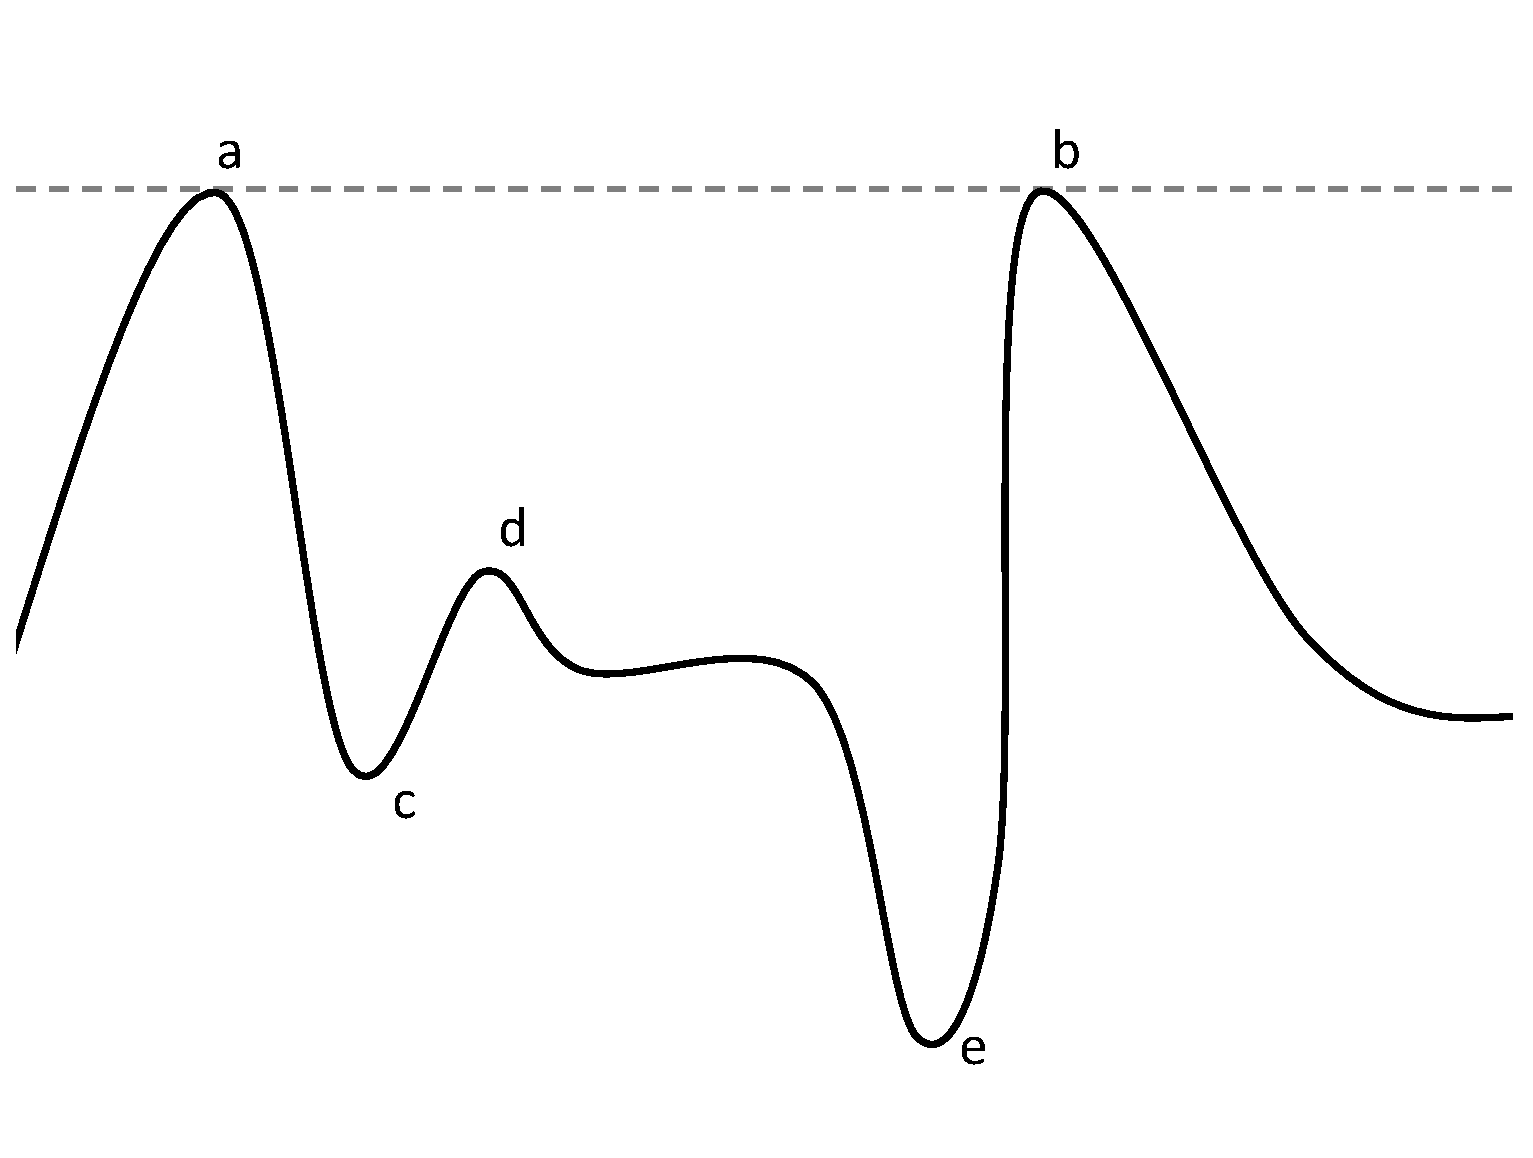
\includegraphics[width=0.6\paperwidth]{searchSpace}
\caption{Examples of local and global optimums.}
\label{localAndGlobalOptims}
\end{figure}


In \ref{localAndGlobalOptims}, we can see different examples of global and local optimums. The points labeled \emph{a} and \emph{b} are both global maximums, as they have the same value. The points
\emph{c} and \emph{d} are respectively local minimum and maximum, while \emph{e} is the global minimum.

A formal definition of the most simple and generic optimization problem would be:

\begin{equation}
min\, f(x)\, s.t.\,(x\in X)
\end{equation}

Where \emph{X} is our search space and \emph{f(x)} the objective function we want to minimize. 

\subsubsection{No Free Lunch Theorem}

\subsubsection{Combinatorial Optimization}

\subsection{Numerical Optimization}
\subsubsection{Linear Programming}
\subsubsection{Quadratic Programming}
\subsection{Nonlinear Programming}

\subsection{Multi-Objective Optimization}

Multi-objective optimization (also called multi-criteria optimization), or MOO, departs significantly from previous categories of optimization in the fact that you have to consider multiple objective functions instead of one. A main aspect of MOO is the way to conciliate these objectives, which are usually contradictory.
An example of real-world everyday MOO problem could be choosing the mean of transportation for a travel, trying to find a balance between speed and cost. Airplane is the fastest way of transportation, but is expensive. While car is slower, it is cheaper. Train is slower than plane, more expensive than car, but can preferred as the best compromise. There still, however, are solutions which are strictly worse than others (in our example, renting an helicopter would probably be both more expensive and slower than buying a seat on a commercial airplane).
From this example, we can see that, for a MOO problem, there rarely is a clear-cut "best" solution. And, more importantly, that even some solutions which are not optimum for \emph{any} of the objectives can be deemed satisfying. 


[[FORMULATION OF A MOO PROBLEM]]

We will now see which strategies have been proposed to deal with such a type of problem.

\subsubsection{Objectives Aggregation}

The first approach is to transform the MOO problem back to a mono-objective optimization problem, by aggregating the different objectives into one.

[[Different strategies : pondered mean, goal programming, min-max -> See thesis JB Welcomme for ref]]

Whatever the chosen aggregation strategy will be, this approach presents severe limitations. 

\subsubsection{Pareto Dominance}

\subsubsection{\emph{A priory} versus \emph{a posteriori} approaches}

\subsection{Multidisciplinary Optimization}

\subsection{Optimization under Uncertainties}

\subsection{Optimization in Dynamic Environments}

\subsubsection{Genetic Algorithms}


\end{document}


%%%%%%%%%%%%%%%%%%%

\Conclusion{Conclusion}
%\Conclusion{Conclusion and Perspectives}

In this thesis we identified a severe limitation of current continuous optimization methods regarding the handling of complex continuation problem. Problems of this category are usually too complex to be solved by classical optimization methods because of multiple factors: the interdependencies of their components, their heavy computational cost, their nonlinearities \emph{etc.} This limitation has been the motivation to propose new specific methods which divide the problem into several disciplines and distribute the optimization process using discipline-level optimizers. However these methods are often difficult to put in practice and cumbersome, not suiting the need of a flexible and iterative process often associated with such problems.

\section*{Thesis Contributions to Continuous Optimization}

This thesis proposes a \textbf{new approach for solving complex continuous problems using an adaptive multi-agent system}. This system, designed following the Adaptive Multi-Agent Systems theory, proposes a decentralized way to automatically distribute the optimization process among the agents, and is able not only to solve large-scale complex problems, but also to adapt to changes made by the user during optimization.\\
The scalability of our approach is made possible by the fact that the agents keep a local view of the system. The system adapts to changes by propagating them from neighbor to neighbor, enabling the \textbf{interactive co-design of the solution}.

This system is built upon a \textbf{general continuous problem modeling we named Natural Domain Modeling for Optimization}, which transform the optimization problem into an entities graph. \textbf{This transformation does not require any simplification, modification or reformulation of the original problem and is fully automatic}.

Following the AMAS theory, we kept the agent perceptions and capabilities at a local level, allowing them to communicate and interact only with their immediate neighbors. Doing so, we are able to handle the problems complexity, as each agent keeps a local point-of-view. The agents are able to use external optimization tools (or can alternatively use local approximation techniques) to solve their local optimization problems. \textbf{This local optimization behavior, along with the message-based global consistency, enables a nominal distributed optimization process}.

We identified several configurations that are susceptible to disturb the good functioning of our system optimization process, corresponding to Non Cooperative Situations (NCS) of the AMAS theory. While these NCS can arise from the interaction of several agents, the agents had to be able to detect and solve them using only local mechanisms. \textbf{For each NCS we proposed local cooperative behaviors for the agents to be able able to cooperatively solve the situation and restore the correct optimization flow}. These cooperative behaviors use specific mechanisms and measures in order to correctly identify the NCS and take the adequate corrective action.

We proved the modularity of our design by showing how our system could be modified to handle additional concerns. To illustrate this, we \textbf{integrated in the agent mechanisms for managing the uncertainties propagation}, effectively allowing the system to realize optimization under uncertainties.

At last, we validated our approach on several test cases. We also integrated our system into a prototype in the context of the ID4CS project funded by the French National Research Agency, prototype currently tested by our industrial parters Airbus and Snecma.

\section*{Thesis Contribution to Multi-Agent Systems}

We already introduced how our identification of specific NCS led to the development of specific agent mechanisms in order for the system to maintain a correct behavior, such as cooperative trajectories, cycle solving \emph{etc.} Based on these NCS and solving mechanisms, we proposed more general Collective Problem Solving Patterns (CPSP). \textbf{These CPSP provide some guidance to the MAS designer regarding some potentially problematic agent configurations which may happen in the system, and propose some solving mechanisms to handle these situations.} We illustrated these CPSP with blueprints summarizing the configuration and mechanisms involved.\\
This work contributes to the ongoing effort of creating general tools for the design of AMAS in the context of problem solving, regrouped under the name AMAS4Opt (Adaptive Multi-Agents Systems for Optimization).

Using the Make Agents Yourself framework, we proposed \textbf{a modular agent architecture adapted to the modeling of hierarchical AMAS agent roles}, based on reusable \enquote{building blocks}. This architecture use a composition of stackable \enquote{skills} components, which allows for an efficient implementation of the handling of the different NCS by the agents.\\
This architecture can be used by the MAS designer as a base to design his own agents, using existing components, and contribute to the effort of providing tools for MAS engineering.

We proposed \textbf{a general graph representation of continuous optimization problems, which can be re-used by MAS designers as a common base to propose other MAS-based approaches for continuous optimization}. Using this common representation, such methods will be easier to compare in terms of solving mechanisms and performances.

\section*{Scientific Perspectives}

\subsection*{Perspectives on MAS for Continuous Optimization}

In regard of continuous optimization, our system could be enhanced with several additional capabilities. Currently, our system concentrates on providing \emph{one} optimal solution. An obvious improvement would be to modify the agents to explore the Pareto front and provide several optimal solutions to the problem. A possible lead would be to modify the objective agents handling of criticality, in order to modulate the weight associated with each objective.

Another possible improvement for designers would be to integrate multi-fidelity models in the system. Multi-fidelity model is a technique to reduce the computational cost of optimization, using several versions of the same model with different computational costs. The low-cost, imprecise models are used at the start of the optimization process, while the high-cost, high-fidelity models are used when the system is starting to converge, in order to improve the precision of the solution. A difficulty of such mechanisms is the maintaining of the consistency between the different levels. This kind of mechanisms could be implemented in our system through the behavior of model agents.

The use of external optimizers could be improved by providing automated optimizer selection mechanisms, in order for the agents to be able to select the most appropriate optimizer, or even change of optimization method during the solving process. Such improvement would possibility require the creation of an optimization ontology in order to characterize the different optimizers.

One could imagine to add self-organizing capabilities to the system, in order to automatically compose the agent graph representing an optimization problem. Such functionality could be used, for example, to provide assistance to the designer during the specification of the optimization problem.\\
With such mechanisms, the user would only have to define a base of elements (variables, models, criteria \emph{etc.}) and the system would be able to automatically assemble the elements into an agent graph, possibly creating (or requesting to the user) new elements as needed. Such functioning would be made possible more easily by the fact that the NDMO formalism does not necessitate any specific formulation to be valid.

\subsection*{Perspectives on the Design of MAS and CPSP}

Concerning the design of MAS, we believe that both researchers and engineers would benefit greatly from the creation of an agent patterns repository. We intend to provide a more detailed and standardized description of the Collective Problem Solving Patterns we identified, with the goal of having a self-sufficient specification document.

An obvious continuation of this work is the identification of new CPSP, either concerning configurations we failed to identify in our application, or with configuration which appear in other application domains. Another possibility concerns the development of alternate handling mechanisms for existing CPSP.

An interesting addition to the CPSP would be to provide an implementation of specialized components which only need to be completed by providing specific functions based on the application domain. To which extend such partial instantiation of the CPSP is possible is an open question at this moment.

\subsection*{Perspectives on the AMAS Theory}

At last, we would like to finish by discussing some interesting observations concerning the AMAS theory in itself and the identification of NCS. Prior works using the AMAS theory concentrated on the identification of NCS at a given moment. The detection of the NCS was usually done immediately by the agents, and the corrective actions were relatively simple and direct.

Most of the NCS we identified were quite different in their functioning. These NCS not only require the agents to cooperate over several iterations to be solved, but their identification itself requires the agents to take additional measures. Moreover, some of the configurations we identified are not systematically problematic in themselves, but only \emph{potentially} problematic depending on some of the parameters (naturally converging cycles, hidden dependencies with adequate influences \emph{etc.}). The common point among these situations is how they are related to the \emph{dynamics} of the system, about its evolution toward one direction or another.

This observation leads to the question of whether a possible distinction could be made between \emph{spatial} NCS, corresponding to the interactions between agents at a given instant, and \emph{temporal} NCS, corresponding to the evolution of an agent over time. If such distinction proved to be relevant, it could lead to new insights on the design of AMAS-based systems, and possibly on the AMAS theory in itself.



%%%%%%%%%%%%%%%%%%%

\appendix
\Partie{Annexes}

%\chapter{Une annexe}

%%%%%%%%%%%%%%%%%%%

\bibliographystyle{plainnat-fr}
\Bibliographie{example}

%%%%%%%%%%%%%%%%%%%

\ListeFigures{Liste des figures}
\ListeTables{Liste des tables}

\end{document}